\chapter{Marco Teórico}
\label{cap:MarcTeorico}

\section{Minería de datos}
\label{sec:dateMine}
A veces llamada como "descubrimiento de información o conocimiento", es el proceso de analizar información de diferentes perspectivas y transformarlo en información de utilidad. Puede ser aplicado a distintas fuentes de datos como: bases de datos, imágenes, internet, etc. Es un campo multidiciplinal que involucra el aprendizaje de máquina, la estadística, bases de datos, la inteligencia artificial y la recuperación de información.\\
Siendo distintos los usos que pueden dársele se pueden generalizar cuatro etapas:\\
\begin{itemize}
\item \textbf{Determinación de objetivos}: Delimitar los objetivos que se esperan alcanzar con el proceso de minado.
\item \textbf{Preprocesamiento de datos}: Se refiere a la limpieza, reducción y transformación de las bases de datos. Es, generalmente, el subproceso que utiliza la mayor cantidad de tiempo.
\item \textbf{Determinación del modelo}: Aplicación de algoritmos para generar un modelo que cumpla los objetivos planteados. Se genera nuevo conocimiento o se descubre un patrón.
\item \textbf{Análisis de los resultados}: Se verifica si el conocimiento es útil.
\end{itemize}

Dentro de las tareas que pueden realizarse utilizando \textit{data mining} pueden encontrarse tales como: Aprendizaje supervisado o clasificación, no supervisado o clustering y reglas de asociación.

	\subsection{Minería de la Web}
	\label{subsec:webMine}
	La aplicación de la minería de datos al contenido que se encuentra en línea es conocida como Minería de la \textit{web} o \textit{web mining}. Se diferencia de la minería de datos tradicional en que ésta última utiliza repositorios de datos; en cambio, la minería \textit{web}, hace uso de información extraída directamente desde la \textit{web}.\\
	Sus métodos son similares en cuanto a sus etapas:
	\begin{itemize}
	\item Selección de las fuentes: referencia al proceso de recuperación de los datos.
	\item Selección y pre-procesamiento: Incluye cualquier transformación o pre-procesamiento que puedan realizárseles a los datos, por ejemplo, eliminar elementos, como palabras, aplicación de correctores de datos, etc.
	\item Generalización: Etapa donde se realiza el proceso de minería en sí. 
	\item Análisis: Desarrolla técnicas para utilizar o visualizar el conocimiento adquirido.
	\end{itemize} 

	La información obtenida puede ser utilizara para analizar tanto el contenido de la web (\textit{Web content mining}) como sus enlaces (o relaciones) (\textit{Web  structure mining}) y/o el registro de navegación de los usuarios (\textit{Web usage mining}).\\

	La primera se refiere a busqueda entre documenos \textit{web} (texto o imágenes), es decir, analiza los documentos y no la relación entre ellos.\\

	La segunda se dedica a analizar la topología de los vínculos existentes y/o analizar la estructura interna de la página \textit{web} y descrbir el \textit{HTML} o el \textit{XML} de la misma.\\

	En particular dentro de la minería de contenido encontramos la minería de texto o \textit{text mining}. Ésta tiene como objetivo el descubrir nueva información a partir colecciones de documentos de texto no estructurado, es decir, texto libre (lenguaje natural, generalmente), aunque también es aceptable otro tipo de información textual como un código fuente. Lo más habitual es trabajar el texto para categorizarlo (Asignar una o más categorías a un documento), clasificarlo (Asignar sólo una clase a un documento) y/o agruparlo (organizar en torno a una jerarquía basado en alguna similitud).\\

	El primer paso para comenzar a trabajar haciendo uso de minería de texto es representar los datos de alguna manera para luego dárselo a los algoritmos adecuados. Algunas de estas representaciones pueden ser las siguientes:
	\begin{itemize}
	\item Bolsas de palabras (\textit{Bag of words}): Representar el texto como un vector de largo n, donde n corresponde al número de palabras, así cada palabra corresponde a un elemento del vector.
	\item Frases: Considera el texto, simplemente, como una frase sintáctica. Así se permite conservar el contexto.
	\item N-gramas: Consideran la información de la posición de la palabra en el texto mediante secuencias de longitud n (n-gramas). 
	\end{itemize}

	Habiendo realizado la representación, el paso siguiente es reducir el conjunto de características. La literatura indica que los métodos más frecuentados son la eliminación de palabras que no aportan información, llevar las palabras a una palabra raíz (\textit{stemming}), entre otros.

\section{Aprendizaje supervisado}
\label{sec:aprendSuperv}
Se caracteriza por ser un proceso de aprendizaje en el que éste se realiza mediante un entrenamiento controlado por un agente externo, el que determina qué respuesta debería generarse a partir de una entrada determinada.\\
Se asocia al concepto de \textit{machine learning} con la minería de datos; la primera busca patrones conocidos y predecir en base a ellos mientras que la segunda busca patrones con anterioridad desconocidos, es decir, la primera tiene una función focalizada en la predicción mientras que la segunda realiza una función exploratoria.\\
Los datos son denominados instancias, ejemplares, casos o vectores, donde una instancia corresponde a cada uno de los datos disponibles para el análisis.\\
Los datos poseen atributos son los elementos dentro de las instancias. Una instancia puede tener asociado un elemento de otro conjunto de atributos llamado "Clase", correspondiente a etiquetas de identificación.\\
Teniendo en cuenta los elementos vistos con anterioridad, se define el objetivo del proceso de aprendizaje como construir una función que relacione las instancias con las clases llamada modelo o, en este caso, clasificador.\\
Se le llama conjunto de entrenamiento al conjunto de datos utilizado para el aprendizaje. Este conjunto es entregado como entrada al algoritmo de aprendizaje y construcción del modelo. Para realizar la evaluación de la calidad del modelo se utiliza un segundo conjunto de instancias llamado datos de validación. Se espera que estos datos no hayan sido vistos con anterioridad por máquina y así obtener la confianza, es decir, la probabilidad de acierto que calcula el sistema para cada predicción.\\

Lo ventajoso de este método es que se podrá clasificar una instancia sin haberla visto nunca, pero la desventaja principal es la que han de utilizarse una gran cantidad de instancias para el proceso de entrenamiento.\\

El proceso de entrenamiento y evaluación se ilustra en la Figura ~\ref{fig:entrenamientoEvaluacion}.

\begin{figure}[!ht]
	\centering
	\captionsetup{justification=centering}
	\includegraphics[scale=0.6]{images/trainTest.png}
	\caption[Proceso de entrenamiento y prueba del modelo.]{Proceso de entrenamiento y prueba del modelo.\\Fuente: Elaboraci\'on propia}
	\label{fig:entrenamientoEvaluacion}
\end{figure}

Dentro de los algoritmos utilizados para la construcción de clasificadores se encuentran \textit{Naïve Bayes} y SVM (\textit{Support Vector Machine}), a continuación se realiza una descripción de ambos. 

	\subsection{Naïve Bayes}
	
	Está basado en el teorema de Bayes, pero asume que independencia entre las variables. 

	\subsection{SVM}


\section{Metodología}
\label{sec:MetodologiaDetalle}

\subsection{Programación Extrema}
\label{subsec:XP}
La Programación Extrema (\textit{Extreme Programming}, XP desde ahora en adelante), comenzó como un proyecto el 6 de Marzo de 1996. Es uno de los procesos ágiles más populares y ha sido provado exitosamente en compañias e industrias de todos los tamaños \cite{xP}.\\
Su éxito se debe a que hace especial incapié en la satisfacción del cliente por sobre la entrega de todo lo el software posible.\\
Aporta cinco formas escenciales para mejorar el proceso de desarrollo de software: Comunicación, simplicidad, retroalimentación, respeto y coraje: Constantemente se comunica al equipo de desarrollo con el cliente. Se intenta mantener el diseño lo más simple y sencillo posible. Se obtiene retroalimentación desde las pruebas desde el día uno. Se les entrega el software al cliente lo más pronto posible con los cambios solicitados. El éxito depende, en gran medida, del respeto y comunicación de los miembros del equipo y los clientes. Implementando XP el equipo puede responder a los cambios sin temor.\\
La metodología implementa unas simples reglas de trabajo, las que se dividen en cinco grandes áreas las que se detallarán a continuación.\\
\begin{enumerate}
\item Planeación:
	\begin{itemize}
	\item Se escriben Historias de usuario. 
	\item Se crea un plan de \textit{releases}.
	\item Se planifican liberaciones pequeñas y frecuentes.
	\item Se divide el proyecto en iteraciones.
	\item Al comienzo de cada iteración se planea cómo será.
	\end{itemize}
\item Manejo:
	\begin{itemize}
	\item Se le da al equipo una área de trabajo.
	\item Se realizan reunione del tipo \textit{stand up meeting} a díario.
	\item Se mide la velocidad del proyecto. 
	\item Se mueven a las personas de sus puestos (para que todo el equipo pueda trabajar en todo).
	\item Se solucionan problemas que instroduzcan quiebres en la metodología.
	\end{itemize}
\item Diseño:
	\begin{itemize}
	\item Simplicidad. El mejor diseño es el más simple.
	\item Se crean \textit{spikes} para reducir el riesgo.
	\item No se agregan funcionalidades antes de tiempo.
	\item Hacer uso de técnicas de \textit{refactoring}, cada vez que sea posible.
	\end{itemize}
\item Implementación:
	\begin{itemize}
	\item El cliente siempre está disponible. 
	\item El código debe ser escrito bajo estándares. 
	\item Se hace uso de \textit{Test Driven Development }(TDD).
	\item Todo el código debe hacerse haciendo uso de \textit{pair programming}.
	\item Sólo una pareja integra código a la vez.
	\item Integración a menudo.
	\item Se cuenta con un equipo dedicado a la integración.
	\item El código es de todos.
	\end{itemize}
\item Prueba:
	\begin{itemize}
	\item Todo el código debe tener pruebas unitarias.
	\item Todas las pruebas deben ser pasadas antes de una liberación.
	\item Cuando se encuentra un \textit{bug}, se crean pruebas.
	\item Los \textit{test} de aceptación se corren a menudo y sus resultados son publicados.
	\end{itemize}
\end{enumerate}

Éstas reglas por si solas pueden carecer de sentido, pero se apoyan en los \textbf{valores} que la metodología quiere entregar y que fueron mencionadas anteriormente, pero ahora son detalladas:

\begin{itemize}
\item Simplicidad: Se hará lo que se solicitó, pero no más. Ésto maximiza el valor entregado dado una fecha límite. Nuestras metas se alcanzarán por medio de pequeños pasos para mitigar errores tan pronto ocurran. Crearemos algo de lo que estemos orgullosos y lo mantendremos en el tiempo a costos razonables.
\item Comunicación: Todos somos partes de un equipo y nos comunicamos cara a cara a diario. Trabajaremos juntos en todo: desde la toma de requerimientos hasta la implementación. Crearemos la mejor solución posible al problema.
\item Retroalimentación: Cada iteración será completada seriamente entregando \textit{software} funcional. Mostraremos nuestro \textit{software} a menudo y prontamente para luego escuchar y aplicar los cambios solicitados. Hablaremos de nuestro proyecto y adaptaremos nuestro proceso a el, no al revéz.
\item Respeto: Todos dan y reciben el respeto que merecen como miembros del equipo. Todos contribuyen con valor así sea simple entusiasmo. Los desarrolladores respetan la experiencia del cliente y viceversa. 
\item Coraje: Diremos la verdad sobre el progreso y nuestras estimaciones. No se documentan excusas por si se falla porque se planea tener éxito. No tenemos porque no trabajamos solos. Nos adaptaremos a los cambio cuando ocurran.
\end{itemize}

El proceso de XP puede puede ser aprecido en la Figura ~\ref{fig:procesoXP}.

\begin{figure}[!ht]
	\centering
	\captionsetup{justification=centering}
	\includegraphics[scale=0.6]{images/flowChartXP.png}
	\caption[Diagrama de flujo de Programación Extrema.]{Diagrama de flujo de Programación Extrema\\Fuente: http://www.extremeprogramming.org/}
	\label{fig:procesoXP}
\end{figure}

\subsection{\textit{Knowledge Discovery in Databases} (KDD)}

Es definido por Fayyad (1996) como "El proceso no trivial de identificar patrones válidos, nuevos, potencialmente útiles y en ultima instancia comprensible en los datos", surge de la necesidad de manejar grandes cantidades de datos e involucra simultaneamente varias disciplinas de investigación tales como el aprendizaje automático, la estadística, inteligencia artificial, sistemas de gestión de bases de datos, sistemas de apoyo a la toma de desiciones, entre otras.\\
Si bien puede variar el usuario, quien es aquel que determina el domino de la aplicación, es decir, cómo se utilizarán los datos, el proceso generalmente considera las siguientes etapas:
\begin{enumerate}
\item Selección de datos: Consiste en buscar el objetivo y las herramientas del proceso de minería, identificando los datos que han de ser extraídos, buscando atributos apropiados de entrada y la información de salida para representar la tarea. Esto quiere decir, primero se debe tener en cuenta lo que se sabe, lo que se quiere obtener y cuáles son los datos que nos facilitarán esa información para poder llegar a nuestra meta, antes de comenzar el proceso como tal.
\item Limpieza de datos: En este paso se limpian los atributos sucios, incluyendo datos incompletos, el ruido y datos inconsistentes. Estos datos sucios, en algunos casos, deben ser eliminados, pues pueden contribuir a un análisis inexacto y resultados incorrectos.
\item Integración de datos: Combina datos de múltiples procedencias incluyendo múltiples bases de datos, que podrían tener diferentes contenidos y formatos.
\item Transformación de datos: Consiste en modificaciones sintácticas llevadas a cabo sobre los datos sin que suponga un cambio en la técnica de minería aplicada. Tiene dos caras, por un lado existen ventajas en el sentido de mejorar la interpretación de las reglas descubiertas y reduce el tiempo de ejecución, por el otro puede llevar a la pérdida de información.
\item Reducción de datos: Reducción del tamaño de los datos, encontrando características más significativas dependiendo del objetivo del proceso.
\item Minería de datos: Consiste en la búsqueda de patrones de interés que puedan expresarse como un modelo o dependencia de los datos. Se ha de de especificar un criterio de preferencia para seleccionar un modelo de un conjunto de posibles modelos. Además se ha de especificar la estrategia de búsqueda (algoritmo), a utilizar.
\item Evaluación de los patrones: Se identifican patrones interesantes que representan conocimiento utilizando diferentes técnicas incluyendo análisis estadísticos y lenguajes de consulta.
\item Interpretación de resultados: Consiste en entender resultados de análisis y sus implicaciones y puede llevar a regresar a algunos pasos anteriores.
\end{enumerate}

La representacíón del proceso puede verse en la Figura ~\ref{fig:procesoKDD}.

\begin{figure}[!ht]
	\centering
	\captionsetup{justification=centering}
	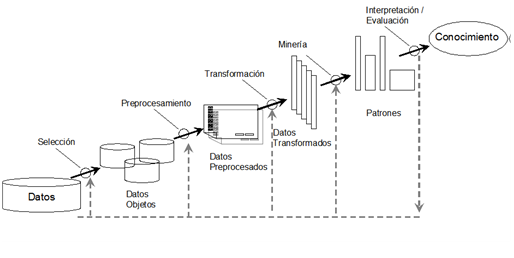
\includegraphics[scale=1]{images/kdd.png}
	\caption[Proceso KDD.]{Proceso KDD\\Fuente: http://mineriadatos1.blogspot.cl/}
	\label{fig:procesoKDD}
\end{figure}



\section{Herramientas}

	\subsection{Play Framework}

	Es un \textit{framework} de código abierto para aplicaciones \textit{web} escrito en \textit{Java} y \textit{Scala}, el cual sigue el patrón de arquitectura \textit{Modelo-Vista-Controlador} (MVC). Utiliza el paradigma de diseño "Convención sobre configuración", el cual apunta a reducir la toma de desiciones que debe tomar el desarrollador sin perder flexibilidad. \\
	Se enfoca en la productividad a aplicaciones \textit{RESTful}.\\
	Elimina la desventaja de desarrollo al utilizar \textit{Java} dada por el continuo ciclo de compilar-empaquetamiento-despliegue. Al detectar cambios en el código realiza inmediatamente la compilación y actualiza en la JVM sin necesidad de reiniciar el servidor.\\
	Play no utilizar sesiones en su funcionar, privilegiando el uso de almacenamiento \textit{offline} o el uso de peticiones \textit{Ajax} para resolver problemas del lado del cliente.

	\subsection{Apache Storm}

	Apache Storm es un sistema de computación en tiempo real de código abierto. Simplifica el problema de flujos (\textit{streams}), de datos sin que estos tengan fin.\\
	Es escalable, tolerante a fallos y garantiza que toda la información será procesada. Presenta \textit{Benchmarks} que señalan que por nodo es capaz de procesar más de un millón de tuplas por segundo.\\
	Se compone principalmente de dos partes. La primera es denominada \textit{Spout} y es la encargada de recoger el flujo de datos de entrada. La segunda es denominada \textit{Bolt} y es la encargada de la transformación o procesado de los datos.\\
	Oficialmente es representado como puede verse en la Figura ~\ref{fig:stormBeLike}. donde los \textit{Spouts} son representados simulando ser llaves de agua desde donde fluyen los datos al sistema y los \textit{Bolts} como rayos donde se procesa el flujo.

	\begin{figure}[!ht]
		\centering
		\captionsetup{justification=centering}
		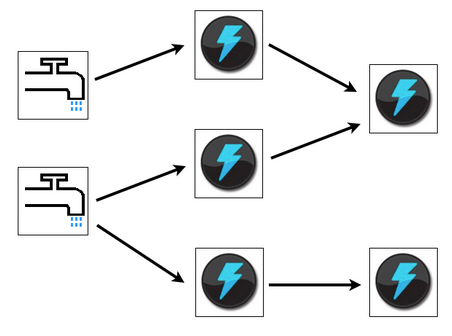
\includegraphics[scale=0.6]{images/stormBeLike.png}
		\caption[Representación del funcionamiento de Apache Storm.]{Representación del funcionamiento de Apache Storm\\Fuente: http://storm.apache.org/}
		\label{fig:stormBeLike}
	\end{figure}

	Uno de los puntos fuertes que tiene este sistema es que al crear una topología donde se instancian \textit{Bolts} y \textit{Spouts}, Storm se encarga de escalar el sistema distribuyendo los elementos en sus componentes.

	\subsubsection{Topología}

	Una topología de Storm es similar a un grafo. Cada nodo se encarga de procesar una determinada información y le pasa el testigo al siguiente nodo. Está compuesta por \textit{Spouts} y \textit{Bolts}.

	\subsubsection{Cluster de Storm}

	Un cluster de Storm no muere, se queda siempre en espera de nuevos datos de entrada mientras el proceso siga activo.
	La arquitectura de Storm se divide en tres componentes:
	\begin{itemize}
	\item Master Node: Ejecuta el demonio llamado Nimbus, el cual es responsable de distribuir el código a través del cluster. Realiza la asignación y monitorización de tareas en las distintas máquinas del cluster.
	\item Worker Node: Ejecutan el demonio Supervisor, el cual se encarga de recoger y procesar los trabajos asignados en la máquina donde está corriendo. En caso de fallo de uno \textit{Worker Node}, Nimbus se dará cuenta y redirigirá el trabajo a otro.
	\item Zookeeper: Si bien no es un componente propio de Storm, es necesario para su funcionamiento, pues se encarga de coordinar Nimbus y Supervisor, además de mantener sus estados, pues ambos son \textit{stateless}.
	\end{itemize}

	\subsubsection{Modos de funcionamiento}

	Storm puede funcionar de dos modos: Local y Cluster. El primero es útil para el desarrollo, pues ejecuta toda la topología en una única JVM, por lo que pueden realizarse fácilmente pruebas de integración, depurar código, etcétera. Este modo simula, haciendo uso de \textit{Threads}, cada nodo del Cluster.\\
	El modo Cluster es considerado el 'modo de producción' y es el modo donde el código es distribuido en máquinas diferentes dentro del Cluster.\\

	\subsubsection{Stream grouping}

	Se refiere a la forma en la que se van a compartir los datos entre los componentes. Como modelo de datos, Storm utiliza tuplas que son listas de valores con un nombre específico. El valor puede ser cualquier tipo, para ello se ha de implementar un serializador.\\

	\begin{itemize}
	\item Shuffle grouping: Storm decide de forma aleatoria la tarea a la que se va a enviar la tupla, de manera que la distribución sea equivalente entre todos los nodos.
	\item Fields gruoping: Se agrupan los \textit{streams} por un determinado campo de manera que se distribuyen los valores que cumplen una determinada condición a la misma tarea.
	\item All grouping: El \textit{stream} pasa por todas las tareas haciendo multicast.
	\item Grobal grouping: El \textit{stream} se envía al \textit{bolt} con ID más bajo.
	\item None grouping: Es un \textit{Shuffle grouping} donde el orden no es importante.
	\item Direct grouping: La tarea es la encargada de decidir hacia donde emitir especificando el ID del destinatario.
	\item Local grouping: Se utiliza el mismo \textit{bolt} si tiene una o más tareas en el mismo proceso.
	\end{itemize}

	\subsection{MongoDB}

	Base de datos no relacional (NoSQL) de código abierto escrita en C++ y está orientada al trabajo en documentos. Lo anterior quiere decir que, en lugar de guardar los datos en registros, lo hace en documentos y éstos son almacenada en una representación binaria de JSON conocida como BSON.\\

	Una de las diferencias fundamentales con respecto a las bases de datos relacionales es que no es necesario que se siga un esquema; en una misma colección - concepto similar a una tabla en las bases de datos relacionales - pueden tener distintos esquemas.\\

	MongoDB fue creado para brindar escalabilidad, rendimiento y disponibilidad. Puede ser utilizado en un servidor único como en múltiples. Esto se logra dado que MongoDB brinda un elevado rendimiento, tanto para lectura como para escritura, potenciando la computación en memoria.\\

	Las consultas en MongoDB se realizan como si se tratase de Javascript entregando como parámetro un objeto JSON. Por ejemplo, dado el documento presentado en la Figura ~\ref{fig:MongoJsonExample}, parte de una colección llamada 'Personas' en MongoDB:

	\begin{figure}[!ht]
		\centering
		\captionsetup{justification=centering}
		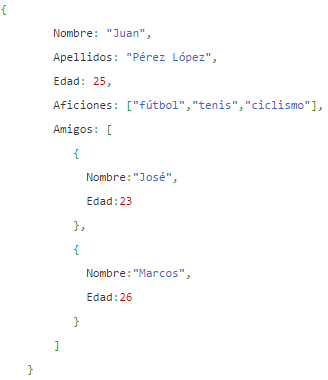
\includegraphics[scale=0.8]{images/MongoJsonExample.png}
		\caption[Documento en MongoDB.]{Documento en MongoDB.\\Fuente: Elaboración propia}
		\label{fig:MongoJsonExample}
	\end{figure}


	Una consulta para encontrar este elemento dentro de la colección se daría de la forma aprecida en la Figura ~\ref{fig:MongoJsonQueryExample}\\

	

	\begin{figure}[!ht]
		\centering
		\captionsetup{justification=centering}
		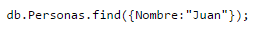
\includegraphics[scale=0.8]{images/MongoJsonQueryExample.png}
		\caption[Consulta en MongoDB.]{Consulta en MongoDB.\\Fuente: Elaboración propia}
		\label{fig:MongoJsonQueryExample}
	\end{figure}


	En pruebas realizando operaciones habituales dentro de las bases de datos el \cite{mongoPerformance} demostró que el tiempo de ejecución de MongoDB, como base de datos NoSQL, aventaja significativamente a las bases de datos relacionales más populares como lo son MySQL y PostgreSQL.


	